\documentclass[a4paper]{article}

\usepackage[english]{babel}
\usepackage[utf8x]{inputenc}
\usepackage{amsmath}
\usepackage{mathtools}
\usepackage{graphicx}
\usepackage{listings}
\usepackage{float}
\usepackage[colorinlistoftodos]{todonotes}

\DeclarePairedDelimiter\ceil{\lceil}{\rceil}
\DeclarePairedDelimiter\floor{\lfloor}{\rfloor}

\title{HW4}
\author{Matthew Flickner, Jeff Fennell, Joseph Barbosa, Misa Pham}

\begin{document}


\maketitle

\section*{1) 4.2(a)}

\begin{figure}[hb]
\centering
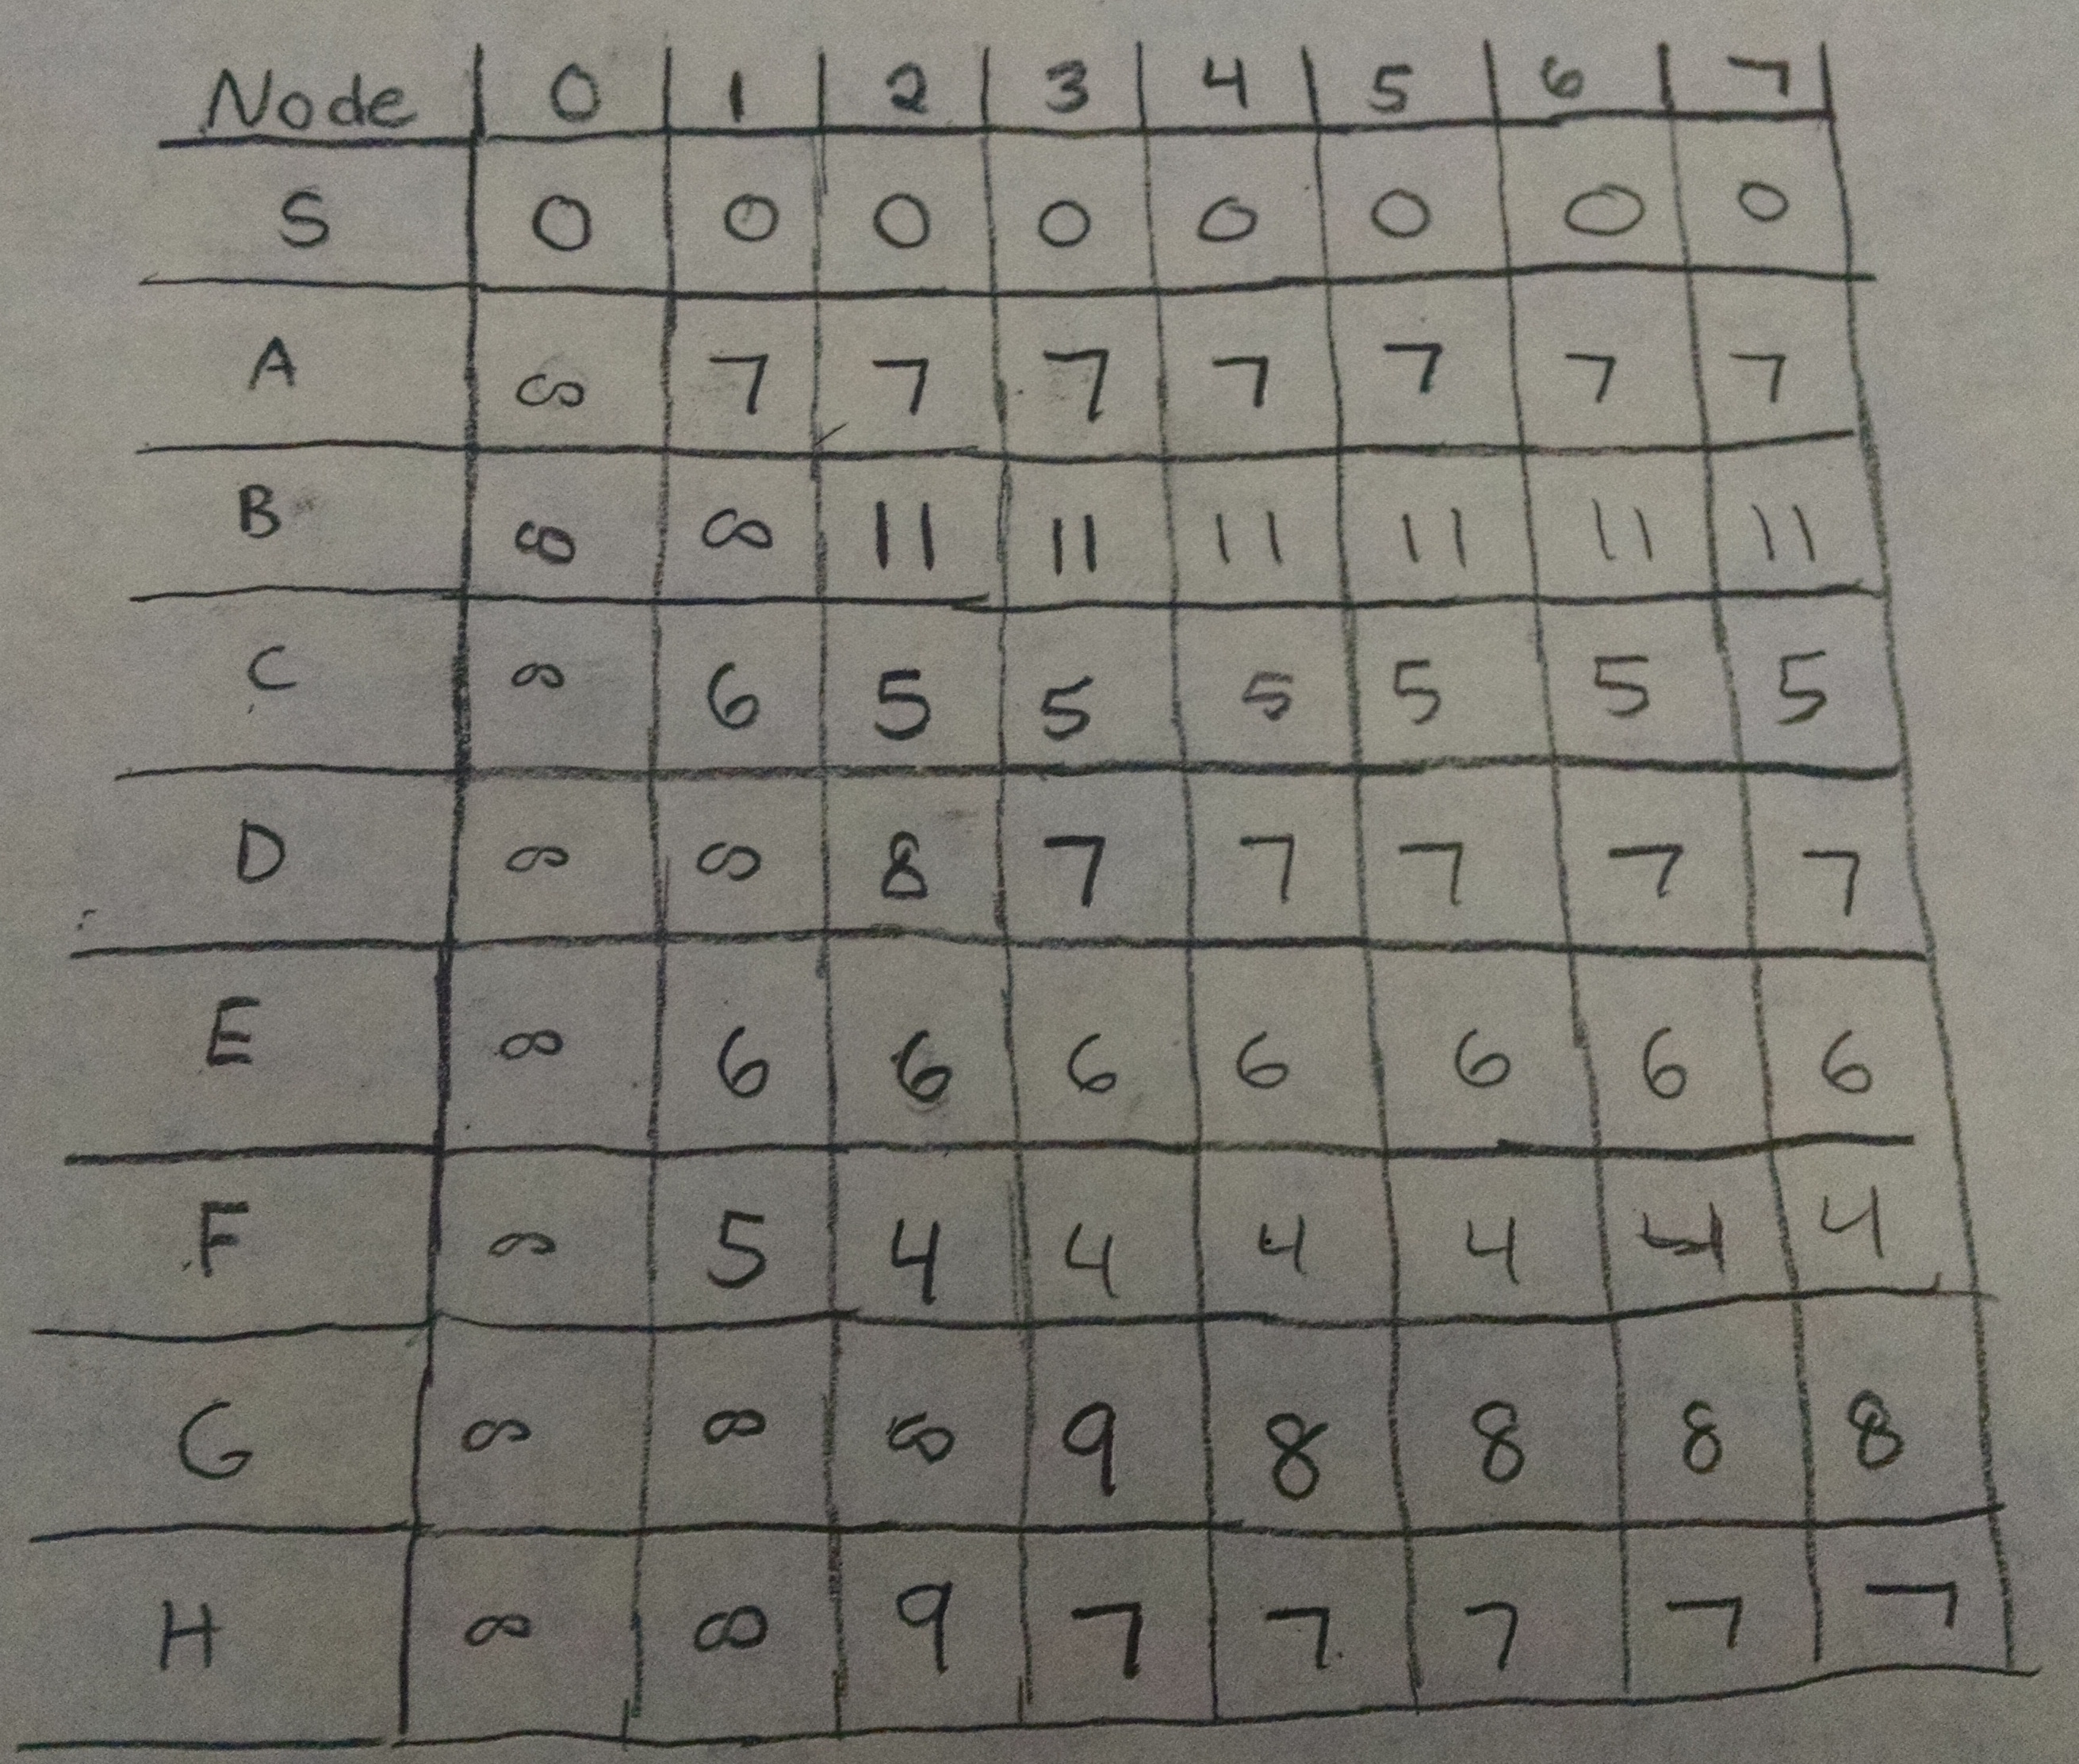
\includegraphics[width=1.0\textwidth]{problem1.jpg}
\end{figure}

\section*{2) 4.8}

\begin{figure}[h]
\centering
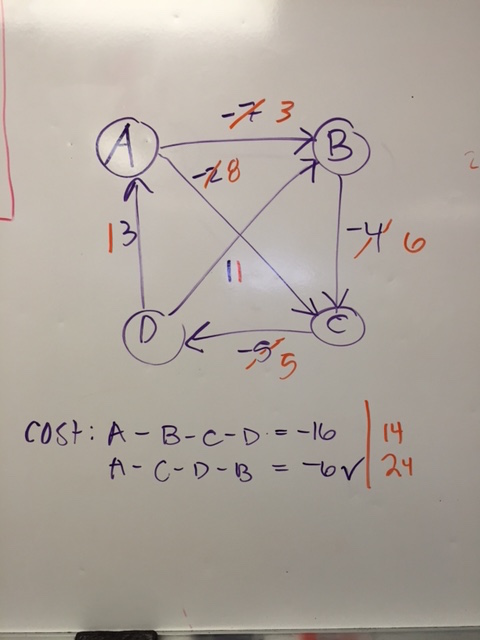
\includegraphics[width=.9\textwidth]{48.JPG}
\end{figure}

Dijkstra's algorithm can only be used with positive integers therefore the negative edges in the graph must be made positive by adding a large positive integer to all the edge values. This is considered a valid method depending on how you view the negative values in terms of weight. If you consider the shortest path to be the path with the lowest negative number (greatest number with a negative sign in front), then this method would be valid. Since the negative values in this case are detracting from the overall weight then they are considered a difference in the length of the path so when a large positive integer is added to the edges this difference will remain the same along all paths. Therefore, the shortest path will also remain the same. On the other hand, if you consider the shortest path to be the path with the higher negative number (smallest number with a negative sign in front), then this method is invalid. The large integer added to the edges turns the smaller negative values into greater positive integers, thus making the previously determined shortest path invalid.  

\section*{3) 4.17a}
Given the bound O\textit{(W$\left|V\right| + \left|E\right|$)} we find that the upper bound is only O\textit{(W$\left|V\right|$)} because the maximum edge weight is W and the vertices will only be updated $\left|V\right|$ - 1 times. This can be accomplished by using Dial's implementation where buckets are used to store vertices and their temporary weights as the shortest path is computed.

Given a Graph $G=(V, E)$, edge weights l, W = max edge weight, vertex s $\in V$
For each vertex in our set of vertices, initialize the variables.

for all vertices v in V:
$dist(v) = \infty$
$prev(v) = nil$
$bucket(v) = nil$

We are creating an array to store temporary weights, as one would do when implementing Dijkstra's algorithm. We then run through the vertices within our set to find the weight and determine the shortest path to the adjacent vertices. We then store this in our variable called u.

\begin{verbatim}
Create an array called shortestPaths of size W|V|: 
shortestPaths[i] keep vertex of distance label i
shortestPaths[0] = s, dist(s)=0, bucket(s)=0
index = 0

while index W|V|:
Increment index:
shortestPaths[index] > O
u = shortestPaths[index]
\end{verbatim}

We will use this u, which is our previously determined index in the array shortestPaths, to go into our implementation of Dijkstra's algorithm for all of the edges in our graph.

\begin{verbatim}
for all edges (u,v) in E:
temp = dist(v)
if dist(v) > dist(u) + l(u,v):
dist(v) = dist(u)+l(u,v)
prev(v) = u
shortestPaths[dist(v)] = v
if temp not equal to inifinity:
Remove v from shortestPaths[temp]
\end{verbatim}


\section*{4) 5.2a}
\begin{figure}[H]
\centering
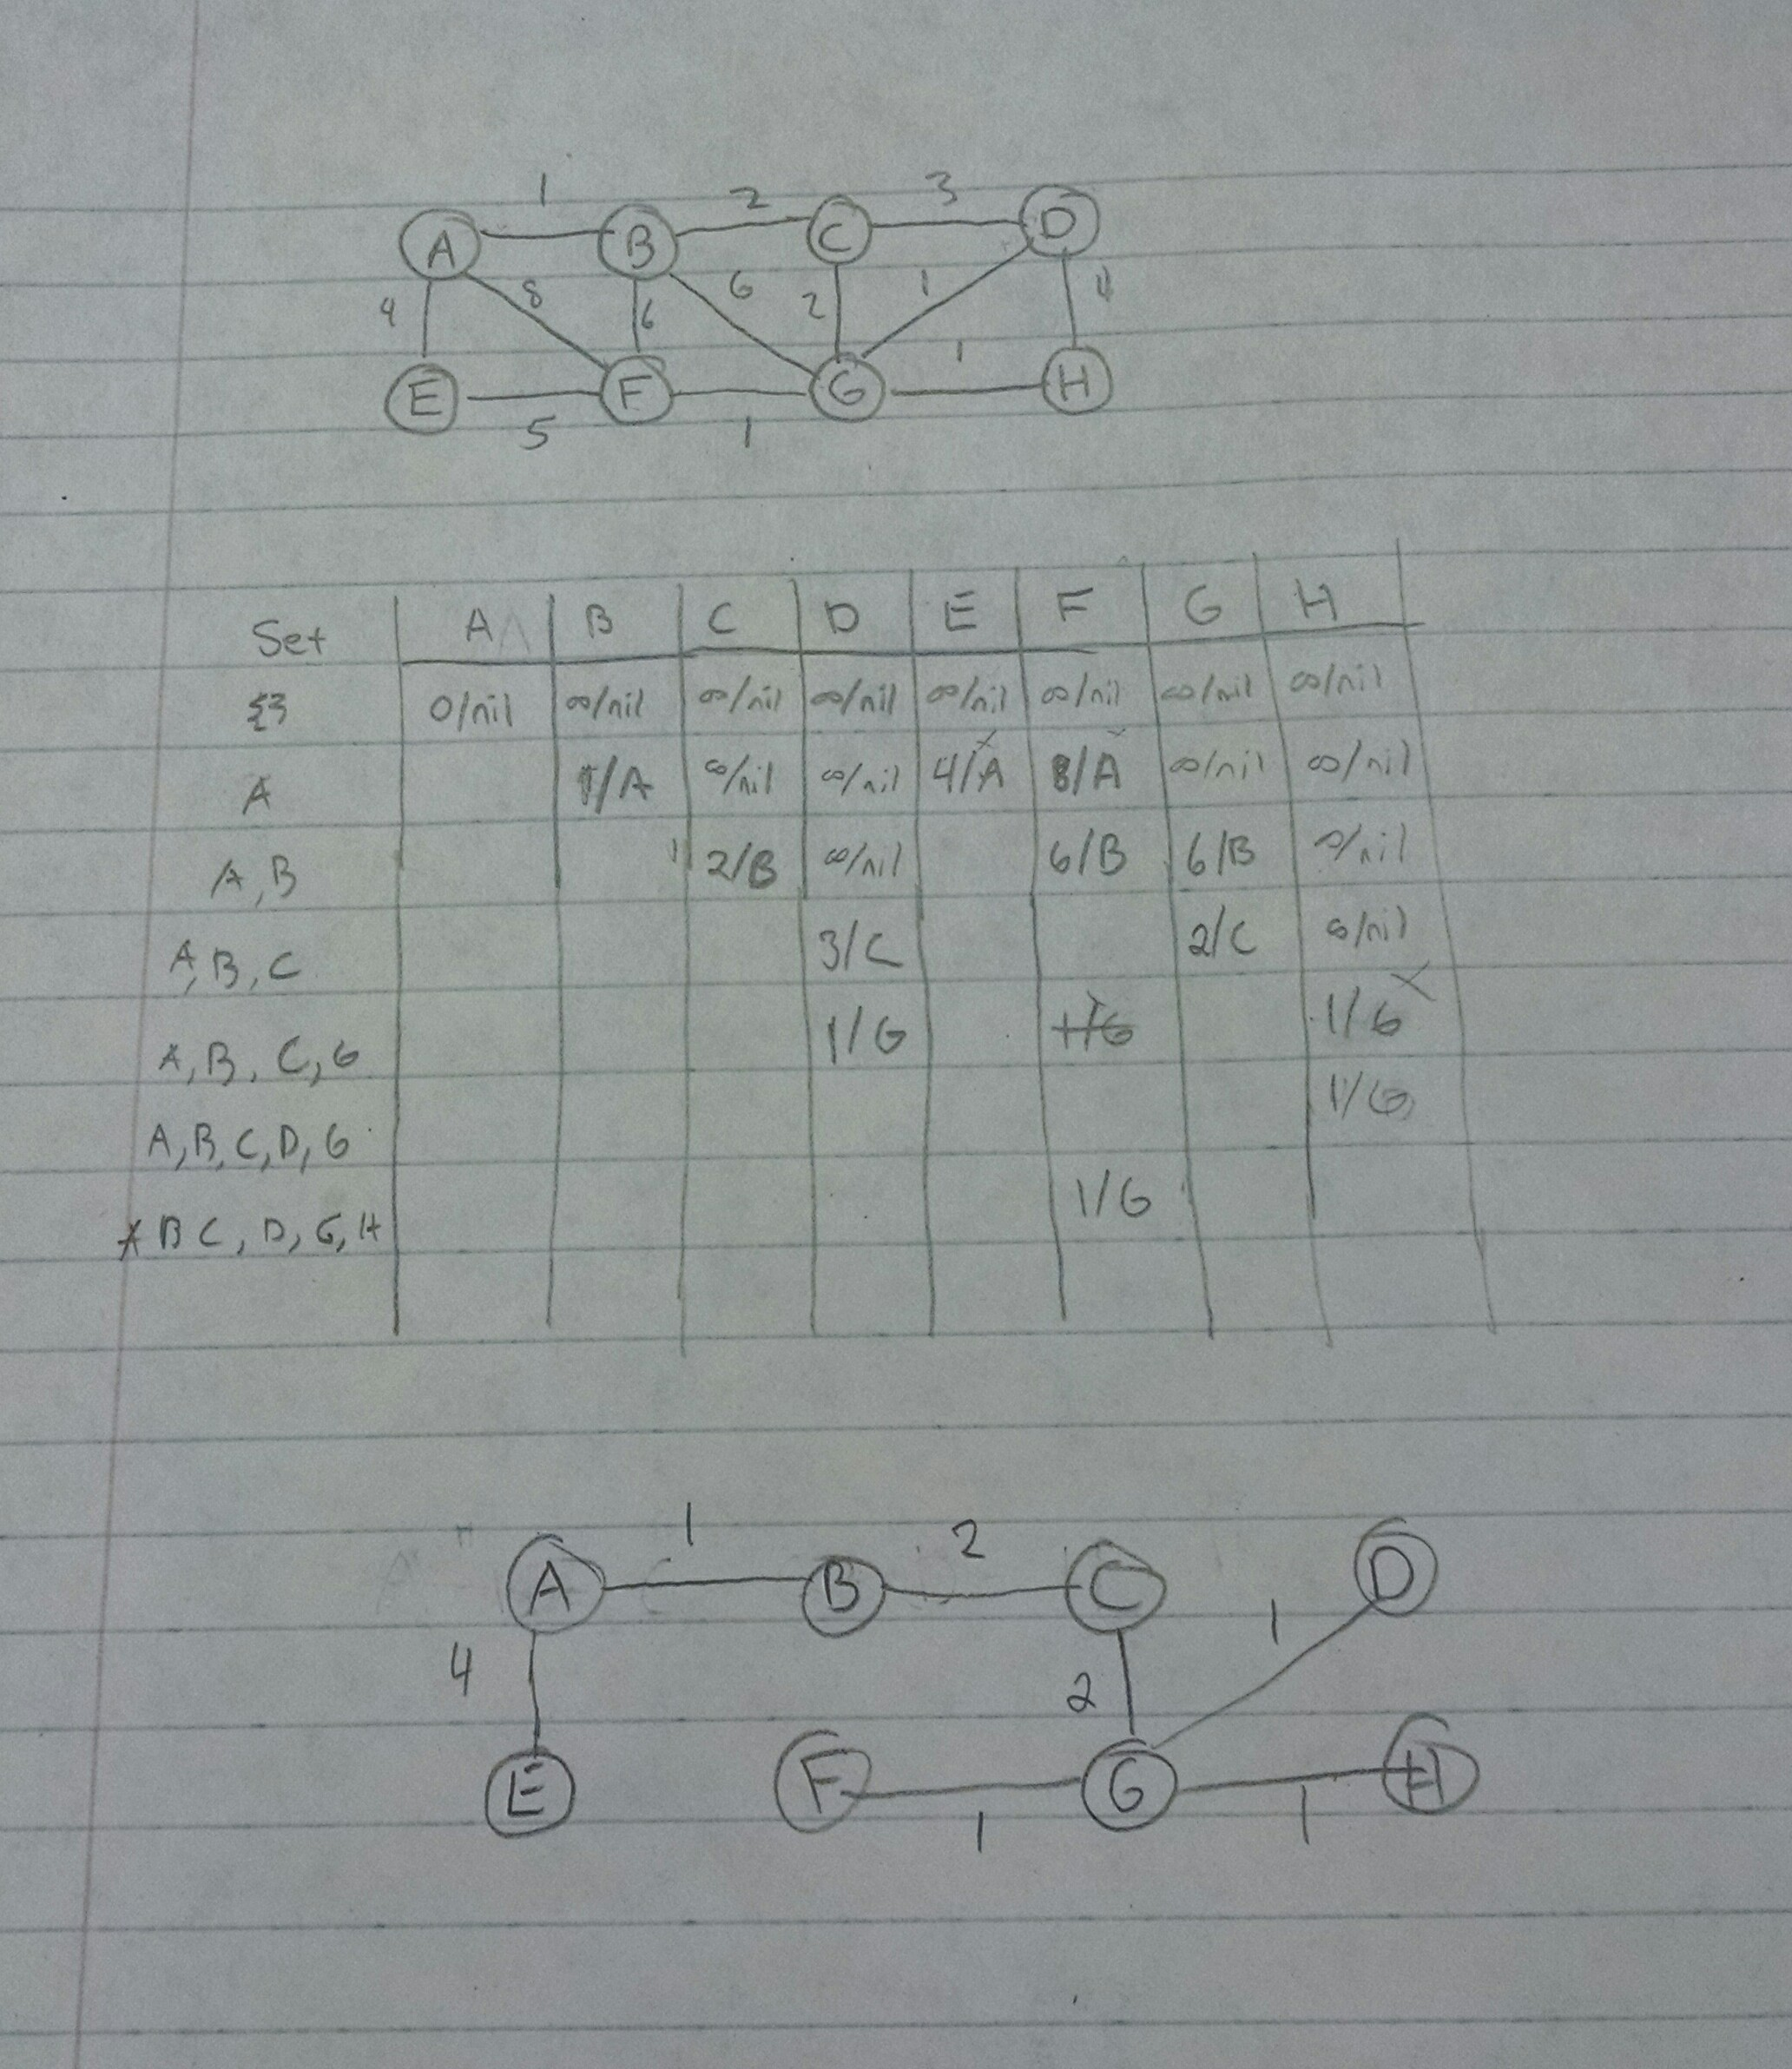
\includegraphics[width=0.9\textwidth]{Prims.jpg}
\end{figure}

\section*{4) 5.2b}
\begin{figure}[H]
\centering
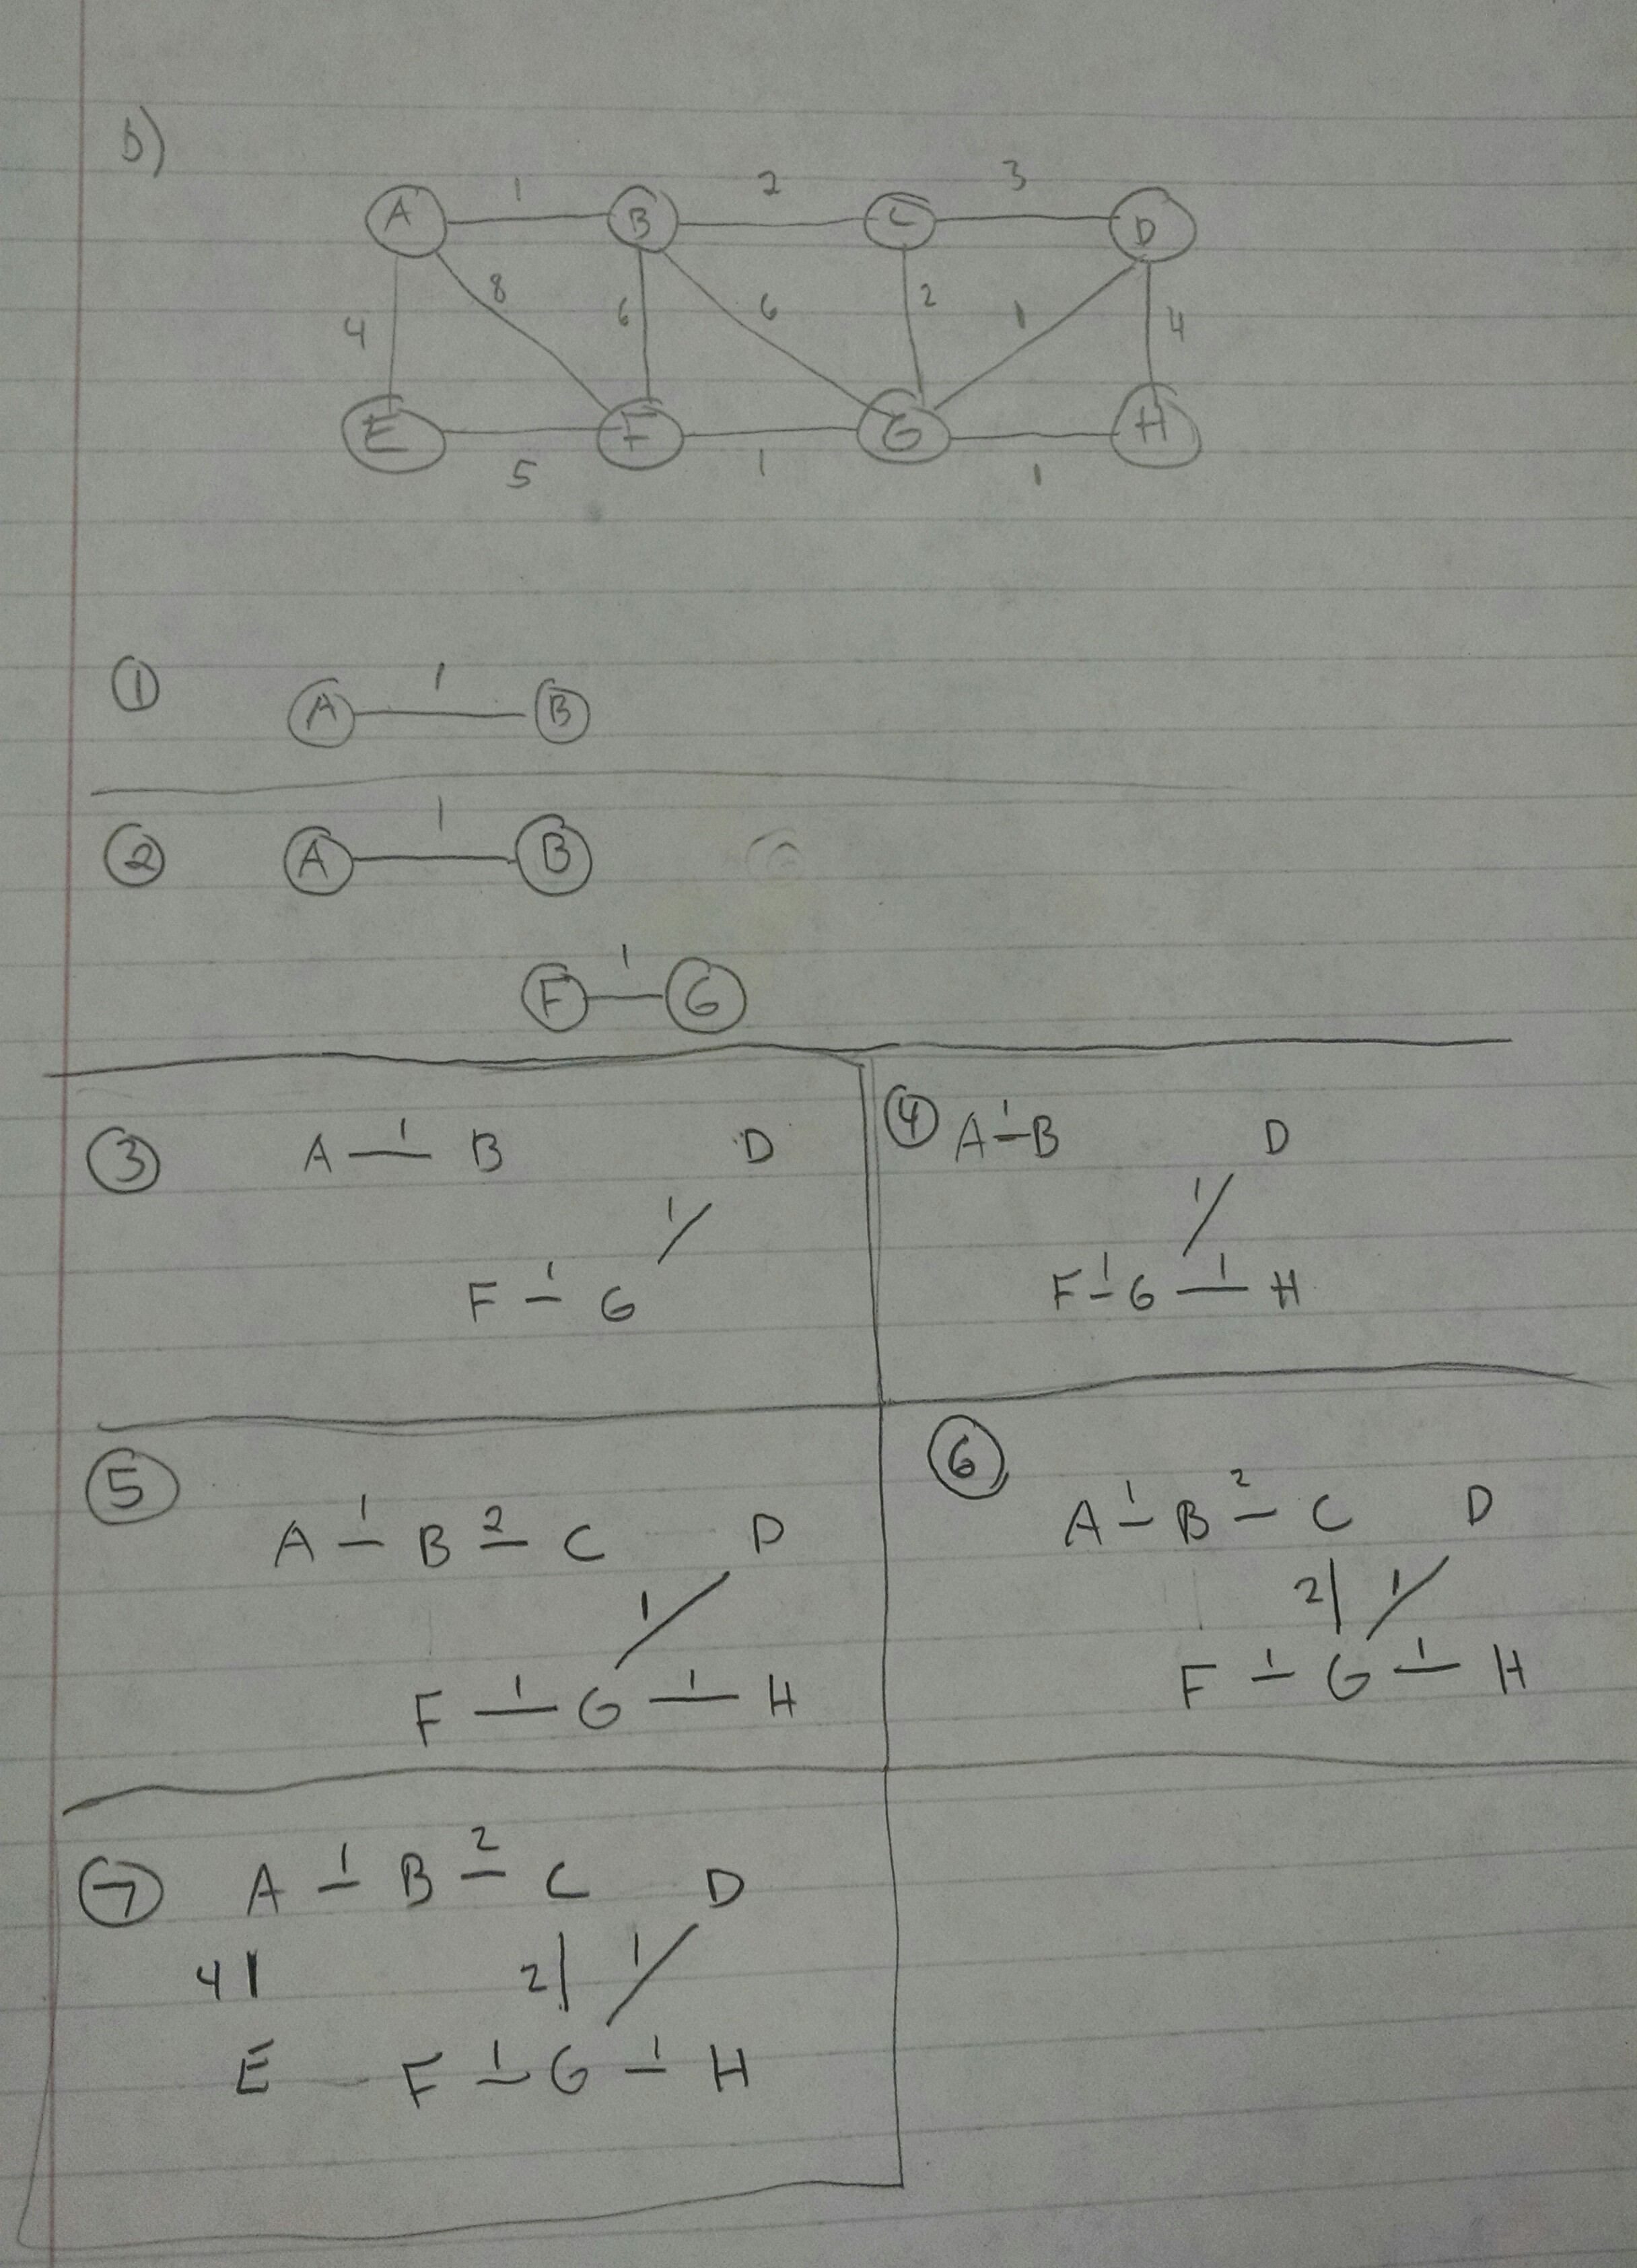
\includegraphics[width=0.9\textwidth]{Kruskal.jpg}
\end{figure}


\section*{5 Subset Sum}
\lstinputlisting[language=Java]{SubsetSum.java}

\section*{6 Kirkman}
\lstinputlisting[language=Java]{KirkmanRow.java}
\lstinputlisting[language=Java]{KirkmanDay.java}



\end{document}
